\section{중간고사 예제}
\subsection{CHAPTER 1. 수학적 모델링과 공학 문제의 해결}
\subsubsection{연습문제 1.18}
속도는 다음 식과 같이 거리 $x (m)$에 대한 시간의 변화량과 같다.
\begin{equation}
\frac{dx}{dt}=v(t)
\end{equation}
\begin{itemize}
\item[(a)] 다음식을 대입하여 시간의 함수로 거리를 표현할 수 있도록 해석해를 구하라.
\begin{displaymath}
v(t)=\frac{gm}{c}\left(1-e^{-(c/m)t}\right)
\end{displaymath}
\item[(b)] 낙하산병문제와 같은 매개변수를 사용하고, Euler법을 사용하여 수치적으로 적분함으로써 처음 10초 동안의 속도와 낙하한 거리를 시간의 함수로 구하라.
\end{itemize}

\subsection{CHAPTER 4. 절단오차와 Taylor 급수}
\subsubsection{연습문제 4.5}
다음과 같은 함수에서 $f(3)$을 계산하기 위해, $x=1$을 기준점으로 0차부터 3차까지의 Taylor급수전개를 사용하여 $f(3)$의 값을 구하라. 참백분율 상대오차 $\epsilon_{t}$를 구하라
\begin{displaymath}
f(x)=25x^3-6x^2+7x-88
\end{displaymath}
\subsubsection{연습문제 4.10}
낙하산병의 속도는 다음과 같이 주어졌다.
\begin{displaymath}
v(t)=\frac{gm}{c}\left(1-e^{-(c/m)t}\right)
\end{displaymath}
\begin{itemize}
\item[(a)] $g=9.8$,$m=50$,$c=12.5\pm1.5$일 때, $t=6$에서 1차 오차해석으로 속도의 추정오차값을 구하도록 하라.
\item[(b)] $g=9.8$,$t=6$,$c=12.5\pm1.5$,$m=50\pm2$로 주어졌을때 1차 오차해석으로 속도의 추정오차값을 구하도록 하라.
\end{itemize}

\subsection{CHAPTER 5. 구간법}
\subsubsection{연습문제 5.2}
다음 식의 실근을 구하라
\begin{displaymath}
f(x)=4x^3-6x^2+7x-2.3
\end{displaymath}
\begin{itemize}
\item[(a)] 이분법을 사용하여 근을 구하라, $x_l =0$과 $x_{u}=1$을 초기구간으로 가정하고, 근사오차 $\epsilon_{a}$가 $10\%$이하로 떨어질 때까지 반복하라
\item[(b)] 가위치법을 사용하여 근을 구하라, 조건은 (a)와 동일
\end{itemize}

\subsubsection{연습문제 5.7}
다음 식의 실근을 구하라
\begin{displaymath}
f(x)=(0.8-0.3x)/x
\end{displaymath}
\begin{itemize}
\item[(a)] 해석적인 방법으로 구하라
\item[(b)] 1과 3을 초기구간으로 하고 가위치법을 세 번 반복해서 실근을 구하라. 각 반복계산 후 근사오차 $\epsilon_{a}$와 참오차 $\epsilon_{t}$를 구하라.
\end{itemize}

\subsubsection{연습문제 5.20}
Figure~\ref{fig:p5-20}(a)는 선형적으로 증가하는 분포하중을 받고 있는 보를 나타낸 것이다. 이에 따른 탄성곡선의 방정식은 다음 식(\ref{eq:p5-20})과 같다.(결과 Figure~\ref{fig:p5-20}(b) 참조)

\begin{figure}[!hbpt]
\centering
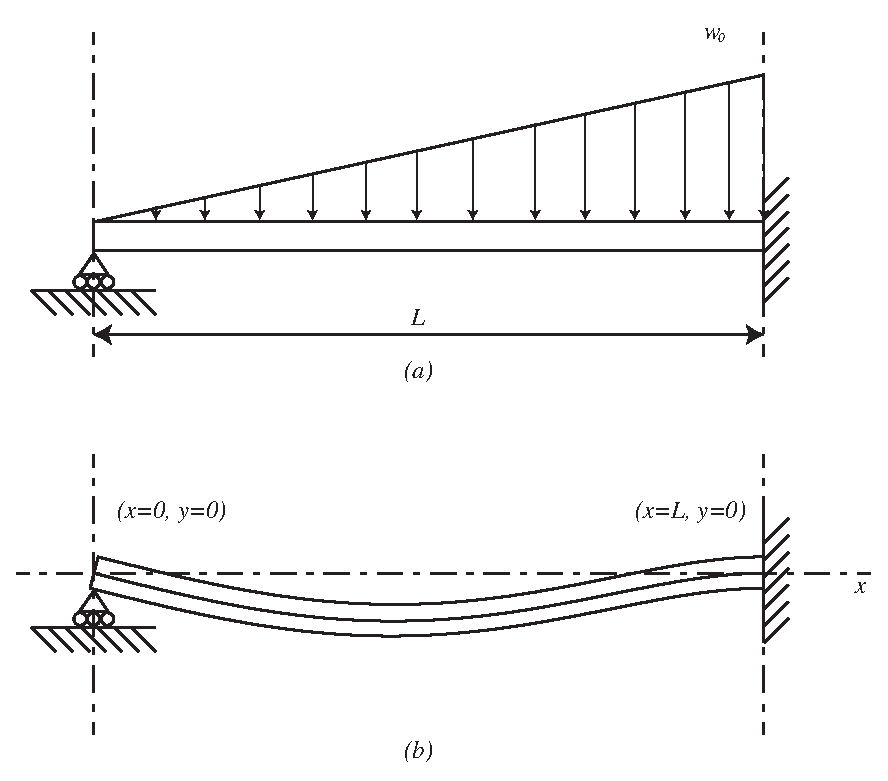
\includegraphics[keepaspectratio=true,width=0.6\linewidth]{figs/5-20.eps}
\caption{선형적으로 증가하는 분포하중을 받고 있는 보}
\label{fig:p5-20}
\end{figure}
\begin{equation}\label{eq:p5-20}
y=\frac{w_{0}}{120EIL}(-x^5 + 2L^2 x^3 - L^4 x)
\end{equation}
이분법을 사용하여 최대 처짐이 발생하는 지점을 구하라(즉, $dy/dx=0$인 $x$의 값). 이 값을 식(\ref{eq:p5-20})에 대입하여 최대 처짐값을 정하라. 매개변수들의 값은 다음과 같다. $L=600cm$, $E=50,000 kN/cm^2$, $I=30,000 cm^4$, $w_{0}=2.5 kN/cm$.

\subsection{CHAPTER 6. 개구간법}
\subsubsection{연습문제 6.2}
다음 함수의 가장 큰 근을 구하라.
\begin{displaymath}
f(x)=2x^3 -11.7x^2 +17.7x-5
\end{displaymath}
\begin{itemize}
\item[(a)] Newton-Raphson법을 사용하라. 초기가정으로 $x_0 =3$을 사용하고 세번 반복하라.
\item[(b)] 할선법을 사용하라. 초기가정으로 $x_{0}=3$, $x_{1}=4$를 사용하고 세번 반복하라.
\item[(c)] 수정된 할선법을 사용하라. 초기가정으로 $x_{0}=3$과 $\delta=0.01$을 사용하고 세번 반복하라.
\end{itemize}
(Newton-Raphson법, 할선법 그리고 수정된 할선법 알고리즘은 각각 아래를 참조.)
\subsubsection{연습문제 6.11}
Newton-Raphson법을 사용하여 다음 식의 근을 구하라
\begin{displaymath}
f(x)=e^{-0.5x}(4-x)-2
\end{displaymath}
초기가정값으로 (a) 2, (b) 6 그리고 (c) 8 을 사용하라. (Newton-Raphson법 알고리즘은 아래를 참조.)

\begin{algorithm}\label{alg:c1}
Let $f:\mathbb{R}\rightarrow\mathbb{R}$ be a differentiable function. The following algorithm computes an approximate solution $x_{r}$ to the equation $f(x)=0$.\\
Choose an initial guess $x_{0}$.
\begin{algorithmic}
\For{$i=0,1,2,\cdots$}
  \If{$f(x_{i})$ is sufficiently small}
    \State $x_{r}=x_{i}$
    \State \Return $x_{r}$
  \EndIf
  \State $x_{i+1}=x_{i}-\frac{f(x_{i})}{f'(x_{i})}$
  \If{$\left|x_{i+1}-x_{i}\right|$ is sufficiently small}
    \State $x_{r}=x_{i+1}$
    \State \Return $x_{r}$
  \EndIf
\EndFor
\end{algorithmic}
\caption{Newton-Raphson Method}
\end{algorithm}

\begin{algorithm}\label{alg:c2}
Let $f:\mathbb{R}\rightarrow\mathbb{R}$ be a differentiable function. The following algorithm computes an approximate solution $x_{r}$ to the equation $f(x)=0$.\\
Choose an initial guess $x_{0}$ and $x_{1}$.
\begin{algorithmic}
\For{$i=0,1,2,\cdots$}
  \If{$f(x_{i})$ is sufficiently small}
    \State $x_{r}=x_{i}$
    \State \Return $x_{r}$
  \EndIf
  \State $x_{i+2}=x_{i+1}-\frac{f(x_{i+1})(x_{i}-x_{i+1})}{f(x_{i})-f(x_{i+1})}$
  \If{$\left|x_{i+2}-x_{i+1}\right|$ is sufficiently small}
    \State $x_{r}=x_{i+2}$
    \State \Return $x_{r}$
  \EndIf
\EndFor
\end{algorithmic}
\caption{Secant Method}
\end{algorithm}

\begin{algorithm}\label{alg:c3}
Let $f:\mathbb{R}\rightarrow\mathbb{R}$ be a differentiable function. The following algorithm computes an approximate solution $x_{r}$ to the equation $f(x)=0$.\\
Choose an initial guess $x_{0}$ and $\delta$.
\begin{algorithmic}
\For{$i=0,1,2,\cdots$}
  \If{$f(x_{i})$ is sufficiently small}
    \State $x_{r}=x_{i}$
    \State \Return $x_{r}$
  \EndIf
  \State $x_{i+1}=x_{i}-\frac{\delta x_{i}f(x_{i})}{f(x_{i}+\delta x_{i})-f(x_{i})}$
  \If{$\left|x_{i+1}-x_{i}\right|$ is sufficiently small}
    \State $x_{r}=x_{i+1}$
    \State \Return $x_{r}$
  \EndIf
\EndFor
\end{algorithmic}
\caption{Modified Secant Method}
\end{algorithm}

\clearpage
\subsection{문제 답안}
\subsubsection{연습문제 1.18(a)}
\begin{align}
\frac{dx}{dt}&=\frac{gm}{c}\left(1-e^{-1(c/m)t}\right)\\
\int_{x(0)}^{x(T)}dx&=\frac{gm}{c}\int_{0}^{T}\left(1-e^{-(c/m)t}\right)dt\\
x(T)-x(0)&=\frac{gm}{c}\left[t+\frac{m}{c}e^{-(c/m)t}\right]_{0}^{T}\\
&=\frac{gm}{c}\left\{T+\frac{m}{c}\left(e^{-(c/m)T}-1\right)\right\}
\end{align}
\subsubsection{연습문제 1.18(b)}
$g=9.8$, $m=68.1$, $c=12.6$을 사용하여 Euler식을 적용하면
\begin{equation}
x_{i+1}=x_{i}+(t_{i+1}-t_{i})\frac{gm}{c}\left(1-e^{-(c/m)t}\right)
\end{equation}

\begin{table}[!hbpt]
\centering
\begin{tabular}{c|c}
\hline\hline
Time(second)&Distance(m)\\
\hline
0&0\\ \hline
1&0\\ \hline
2&8.9468\\ \hline
3&25.3292\\ \hline
4&47.8912\\ \hline
5&75.5889\\ \hline
6&107.555\\ \hline
7&143.0683\\ \hline
8&181.5297\\ \hline
9&222.4413\\ \hline
10&265.3892\\ \hline
\hline
\end{tabular}
\end{table}

\subsubsection{연습문제 4.5}
\begin{displaymath}
f(x)=25x^3-6x^2+7x-88
\end{displaymath}
참값은 $f(3)=554$

\begin{table}[!hbpt]
\centering
\begin{tabular}{c|c|c|c}
\hline\hline
Order&Equation&Result&$\epsilon_{t}$\\
\hline
0&$f(3)\cong f(1)$&$f(3)\cong -62$& 111\%\\
1&$f(3)\cong f(1)+f'(1)(3-1)$&$f(3)\cong 78$ & 86.9\%\\
2&$f(3)\cong f(1)+f'(1)(3-1)+\frac{1}{2!}f''(1)(3-1)^2$&$f(3)\cong354$&36.10\%
\\ \hline\hline
\end{tabular}
\end{table}

\subsubsection{연습문제 4.10(a)}
$g=9.8$,$m=50$,$c=12.5\pm1.5$일 때, $t=6$에서 속도의 1차오차해석에 의한 추정오차값은
\begin{align}
\Delta v(t)&\cong\left|\frac{\partial v(t)}{\partial c}\right|\Delta c\\
&=\left|\frac{gm}{c^2}\left(e^{-(c/m)t}-1\right)+\frac{gt}{c}\left(e^{-(c/m)t}\right)\right|\Delta c\\
&=\left|-\frac{gm}{c}+\frac{g}{c}(\frac{m}{c}+t)e^{-(c/m)t}\right|\Delta c\\
&=\left|-1.2807\right|\Delta c\\
&=1.2807\cdot1.5\\
\therefore v(t)&=35.5133\pm1.9212
\end{align}
\subsubsection{연습문제 4.10(b)}
$g=9.8$,$t=6$,$c=12.5\pm1.5$,$m=50\pm2$일 때, $t=6$에서 속도의 1차오차해석에 의한 추정오차값은
\begin{align}
\Delta v(t)&\cong\left|\frac{\partial v(t)}{\partial c}\right|\Delta c+\left|\frac{\partial v(t)}{\partial m}\right|\Delta m\\
&=\left|-\frac{gm}{c}+\frac{g}{c}(\frac{m}{c}+t)e^{-(c/m)t}\right|\Delta c + \left|\frac{g}{c}-\left(\frac{g}{c}+\frac{gt}{m}\right)e^{-(c/m)t}\right|\Delta m\\
&=\left|-1.2807\right|\Delta c +\left|0.2370\right|\Delta m\\
&=1.2807\cdot1.5+0.2370\cdot2\\
\therefore v(t)&=35.5133\pm2.3951
\end{align}

\subsubsection{연습문제 5.2(a)}
이분법을 사용하여 근을 구하라, $x_l =0$과 $x_{u}=1$을 초기구간으로 가정하고, 근사오차 $\epsilon_{a}$가 $10\%$이하로 떨어질 때까지 반복하라
\begin{table}[!hbpt]
\centering
\begin{tabular}{c|c|c|c|c|c}
\hline\hline
Iter.&$x_{l}$&$x_{u}$&$x_{r}$&$f(x_{r})$&$\epsilon_{a}$\\
\hline
1&0&1&0.5&0.2&-\\
2&0&0.5&0.25&-0.8625&100\%\\
3&0.25&0.5&0.375&-0.30781&33.3333\%\\
4&0.375&0.5&0.4375&-0.050977&14.2857\%\\
5&0.4375&0.5&0.46875&0.074878&6.6667\%\\
\hline\hline
\end{tabular}
\end{table}

\clearpage
\subsubsection{연습문제 5.2(b)}
가위치법을 사용하여 근을 구하라, $x_l =0$과 $x_{u}=1$을 초기구간으로 가정하고, 근사오차 $\epsilon_{a}$가 $10\%$이하로 떨어질 때까지 반복하라
\begin{table}[!hbpt]
\centering
\begin{tabular}{c|c|c|c|c|c}
\hline\hline
Iter.&$x_{l}$&$x_{u}$&$x_{r}$&$f(x_{r})$&$\epsilon_{a}$\\
\hline
1&0&1&0.46&0.039744&-\\
2&0&0.46&0.45219&0.0083076&1.728\%\\
\hline\hline
\end{tabular}
\end{table}

\subsubsection{연습문제 5.7(b)}

\begin{table}[!hbpt]
\centering
\begin{tabular}{c|c|c|c|c|c|c}
\hline\hline
Iter.&$x_{l}$&$x_{u}$&$x_{r}$&$f(x_{r})$&$\epsilon_{a}$&$\epsilon_{t}$\\
\hline
1&1&3&2.875&-0.021739&-&0.078125\%\\
2&1&2.875&2.7969&-0.013966&2.7933\%&0.048828\%\\
3&1&2.7969&2.748&-0.0088842&1.7768\%&0.030518\%\\
\hline\hline
\end{tabular}
\end{table}

\subsubsection{연습문제 5.20}
최대처짐이 발생하는 지점은 $dy/dx=0$인 지점이므로 주어진 식의 1차도함수를 구한다.
\begin{equation}
\frac{dy}{dx}=\frac{w_{0}}{120EIL}\left(-5x^{4}+6L^{2}x^{2}-L^{4}\right)
\end{equation}
즉, 처짐에 대한 함수의 근을 이분법으로 찾는다.
\begin{equation}
f(x)=\frac{w_{0}}{120EIL}\left(-5x^{4}+6L^{2}x^{2}-L^{4}\right)
\end{equation}

\begin{table}[!hbpt]
\centering
\begin{tabular}{c|c|c|c|c|c|c}
\hline\hline
Iter.&$x_{l}$&$x_{u}$&$x_{r}$&$\frac{dy}{dx}$&$y$&$\epsilon_{t}$\\
\hline
1&0&600&300&0.0005625&-0.50625&-\\
2&0&300&150&-0.0019336&-0.39551&100\%\\
3&150&300&225&-0.00076538&-0.4985&33.3333\%\\
4&225&300&262.5&-0.00010423&-0.51489&14.2857\%\\
5&262.5&300&281.25&0.00023088&-0.5137&6.6667\%\\
6&262.5&281.25&271.875&$6.3442\times 10^{-5}$&-0.51508&3.4483\%\\
7&262.5&271.875&267.1875&$-2.0405\times 10^{-5}$&-0.51518&1.7544\%\\
8&267.1875&271.875&269.5313&$2.1521\times 10^{-5}$&-0.51518&0.86957\%\\
\hline\hline
\end{tabular}
\end{table}
\clearpage
\subsubsection{연습문제 6.2(a)}
Newton-Raphson법을 사용하라. 초기가정으로 $x_0 =3$을 사용하고 세번 반복하라.
\begin{table}[!hbpt]
\centering
\begin{tabular}{c|c|c|c|c}
\hline\hline
Iter.&$x_{i}$&$f(x_{i})$&$f'(x_{i})$&$\epsilon_{a}$\\
\hline
0&3&-3.2&1.5&41.5584\%\\
1&5.1333&48.0901&55.6867&20.2256\%\\
2&4.2698&12.9562&27.1724&12.5712\%\\
\hline\hline
\end{tabular}
\end{table}

\subsubsection{연습문제 6.2(b)}
할선법을 사용하라. 초기가정으로 $x_0 =3$을 사용하고 세번 반복하라.
\begin{table}[!hbpt]
\centering
\begin{tabular}{c|c|c|c|c|c}
\hline\hline
Iter.&$x_{i}$&$x_{i+1}$&$f(x_{i})$&$f(x_{i+1})$&$\epsilon_{a}$\\
\hline
0&3&4&-3.2&6.6&20.2454\%\\
1&4&3.3265&6.6&-1.9689&4.445\%\\
2&3.3265&3.4813&-1.9689&-0.79592&2.9279\%\\
\hline\hline
\end{tabular}
\end{table}

\subsubsection{연습문제 6.2(c)}
수정된 할선법을 사용하라. 초기가정으로 $x_0 =3$와 $\delta=0.01$을 사용하고 세번 반복하라.
\begin{table}[!hbpt]
\centering
\begin{tabular}{c|c|c|c|c}
\hline\hline
Iter.&$x_{i}$&$f(x_{i})$&$f(x_{i}+\delta x_{i})$&$\epsilon_{a}$\\
\hline
0&3&-3.2&-3.1493&38.6828\%\\
1&4.8926&35.7632&38.0973&18.0945\%\\
2&4.1429&9.7305&10.7367&10.7055\%\\
\hline\hline
\end{tabular}
\end{table}

\subsubsection{연습문제 6.11}
Newton-Raphson법을 사용하여 다음 식의 근을 구하라
\begin{displaymath}
f(x)=e^{-0.5x}(4-x)-2
\end{displaymath}
초기가정값으로 (a) 2, (b) 6 그리고 (c) 8 을 사용하라. (Newton-Raphson법 알고리즘은 아래를 참조.)

\begin{table}[!hbpt]
\centering
\begin{tabular}{c|c|c|c|c}
\hline\hline
Iter.&$x_{i}$&$f(x_{i})$&$f'(x_{i})$&$\epsilon_{a}$\\
\hline
0&2&-1.2642&-0.73576&609.9294\%\\
1&0.28172&1.2297&-2.4835&63.7376\%\\
2&0.77689&0.18563&-1.7709&11.8884\%\\
3&0.88171&0.0065795&-1.6468&0.45109\%\\
\hline\hline
\end{tabular}
\caption{초기가정값 $x_{0}=2$}
\end{table}

\begin{table}[!hbpt]
\centering
\begin{tabular}{c|c|c|c|c}
\hline\hline
Iter.&$x_{i}$&$f(x_{i})$&$f'(x_{i})$&$\epsilon_{a}$\\
\hline
0&6&-2.0996&0&NaN\%\\
\hline\hline
\end{tabular}
\caption{초기가정값 $x_{0}=6$}
\end{table}

\begin{table}[!hbpt]
\centering
\begin{tabular}{c|c|c|c|c}
\hline\hline
Iter.&$x_{i}$&$f(x_{i})$&$f'(x_{i})$&$\epsilon_{a}$\\
\hline
0&8&-2.0733&0.018316&93.3991\%\\
1&121.1963&-2&2.7731e-25&100\%\\
2&7212131452880262800000000&-2&0&NaN\%\\
\hline\hline
\end{tabular}
\caption{초기가정값 $x_{0}=8$}
\end{table}

\clearpage
\subsubsection{알고리즘 테이블}

\begin{algorithm}\label{alg:c5}
Let $f:\mathbb{R}\rightarrow\mathbb{R}$ be a differentiable function. The following algorithm computes an approximate solution $x_{r}$ to the equation $f(x)=0$.\\
Choose lower $x_{l}$ and upper $x_{u}$ guesses for the root such that the function changes sign over the interval. This can be checked by ensuring that $f(x_{l})f(x_{u})<0$.
\begin{algorithmic}
\While{$f(x_{r})$ is not sufficiently small}
  \State $x_{r}=\frac{x_{l}+x_{u}}{2}$
  \If{$f(x_{l})f(x_{r})<0$}
    \State $x_{u}=x_{r}$
  \Else
    \State $x_{l}=x_{r}$
  \EndIf  
  \If{$\epsilon_{a}=\left|\frac{x_{new}-x_{old}}{x_{new}}\right|$ is sufficiently small}
    \State $x_{r}=x_{new}$
    \State \Return $x_{r}$
  \EndIf
\EndWhile
\end{algorithmic}
\caption{이분법(Bisection Method)}
\end{algorithm}

\begin{algorithm}\label{alg:c5}
Let $f:\mathbb{R}\rightarrow\mathbb{R}$ be a differentiable function. The following algorithm computes an approximate solution $x_{r}$ to the equation $f(x)=0$.\\
Choose lower $x_{l}$ and upper $x_{u}$ guesses for the root such that the function changes sign over the interval. This can be checked by ensuring that $f(x_{l})f(x_{u})<0$.
\begin{algorithmic}
\While{$f(x_{r})$ is not sufficiently small}
  \State $x_{r}=x_{u}-\frac{f(x_{u})(x_l -x_u)}{f(x_l)-f(x_u)}$
  \If{$f(x_{l})f(x_{r})<0$}
    \State $x_{u}=x_{r}$
  \Else
    \State $x_{l}=x_{r}$
  \EndIf  
  \If{$\epsilon_{a}=\left|\frac{x_{new}-x_{old}}{x_{new}}\right|$ is sufficiently small}
    \State $x_{r}=x_{new}$
    \State \Return $x_{r}$
  \EndIf
\EndWhile
\end{algorithmic}
\caption{가위치법(False Position Method)}
\end{algorithm}

\begin{algorithm}\label{alg:c1}
Let $f:\mathbb{R}\rightarrow\mathbb{R}$ be a differentiable function. The following algorithm computes an approximate solution $x_{r}$ to the equation $f(x)=0$.\\
Choose an initial guess $x_{0}$.
\begin{algorithmic}
\For{$i=0,1,2,\cdots$}
  \If{$f(x_{i})$ is sufficiently small}
    \State $x_{r}=x_{i}$
    \State \Return $x_{r}$
  \EndIf
  \State $x_{i+1}=x_{i}-\frac{f(x_{i})}{f'(x_{i})}$
  \If{$\left|x_{i+1}-x_{i}\right|$ is sufficiently small}
    \State $x_{r}=x_{i+1}$
    \State \Return $x_{r}$
  \EndIf
\EndFor
\end{algorithmic}
\caption{Newton-Raphson Method}
\end{algorithm}

\begin{algorithm}\label{alg:c2}
Let $f:\mathbb{R}\rightarrow\mathbb{R}$ be a differentiable function. The following algorithm computes an approximate solution $x_{r}$ to the equation $f(x)=0$.\\
Choose an initial guess $x_{0}$ and $x_{1}$.
\begin{algorithmic}
\For{$i=0,1,2,\cdots$}
  \If{$f(x_{i})$ is sufficiently small}
    \State $x_{r}=x_{i}$
    \State \Return $x_{r}$
  \EndIf
  \State $x_{i+2}=x_{i+1}-\frac{f(x_{i+1})(x_{i}-x_{i+1})}{f(x_{i})-f(x_{i+1})}$
  \If{$\left|x_{i+2}-x_{i+1}\right|$ is sufficiently small}
    \State $x_{r}=x_{i+2}$
    \State \Return $x_{r}$
  \EndIf
\EndFor
\end{algorithmic}
\caption{Secant Method}
\end{algorithm}

\begin{algorithm}\label{alg:c3}
Let $f:\mathbb{R}\rightarrow\mathbb{R}$ be a differentiable function. The following algorithm computes an approximate solution $x_{r}$ to the equation $f(x)=0$.\\
Choose an initial guess $x_{0}$ and $\delta$.
\begin{algorithmic}
\For{$i=0,1,2,\cdots$}
  \If{$f(x_{i})$ is sufficiently small}
    \State $x_{r}=x_{i}$
    \State \Return $x_{r}$
  \EndIf
  \State $x_{i+1}=x_{i}-\frac{\delta x_{i}f(x_{i})}{f(x_{i}+\delta x_{i})-f(x_{i})}$
  \If{$\left|x_{i+1}-x_{i}\right|$ is sufficiently small}
    \State $x_{r}=x_{i+1}$
    \State \Return $x_{r}$
  \EndIf
\EndFor
\end{algorithmic}
\caption{Modified Secant Method}
\end{algorithm}
